\documentclass[10pt]{article}
\usepackage{amsmath}
\usepackage{amsfonts}
\usepackage{graphicx}
%\usepackage{epstopdf}
\usepackage{hyperref}
\usepackage[left=.9in,right=.9in,top=.7in,bottom=.7in]{geometry}
%\usepackage[left=1.1in,right=1.1in,top=.7in,bottom=.7in]{geometry}
\usepackage{multirow}
\usepackage{verbatim}
\usepackage{fancyhdr}
\usepackage[small,compact]{titlesec} 
\usepackage{color}
\usepackage{ulem}
\usepackage{natbib}
\renewcommand{\cite}{\citet}

%\usepackage[screen,nopanel,gray]{pdfscreen}
%\screensize{4in}{5.33in}
%\margins{0.75in}{0.75in}{0.75in}{0.75in}


%\usepackage{pxfonts}
%\usepackage{isomath}
%\usepackage{mathpazo}
%\usepackage{arev} %     (Arev/Vera Sans)
%\usepackage{eulervm} %_   (Euler Math)
%\usepackage{fixmath} %  (Computer Modern)
%\usepackage{hvmath} %_   (HV-Math/Helvetica)
%\usepackage{tmmath} %_   (TM-Math/Times)
%\usepackage{cmbright}
%\usepackage{ccfonts} \usepackage[T1]{fontenc}
%\usepackage[garamond]{mathdesign}

\newcommand{\argmax}{\operatornamewithlimits{arg\,max}}
\newcommand{\argmin}{\operatornamewithlimits{arg\,min}}
\newcommand{\myTable}[1]{\begin{table}[b]\caption{#1}
    \begin{minipage}{\linewidth} \begin{center}}
\newcommand{\myTableEnd}{\end{center}\end{minipage}\end{table}}

\def\inprobLOW{\rightarrow_p}
\def\inprobHIGH{\,{\buildrel p \over \rightarrow}\,} 
\def\inprob{\,{\inprobHIGH}\,} 
\def\indist{\,{\buildrel d \over \rightarrow}\,} 

\newtheorem{theorem}{Theorem}

%\pagestyle{fancy}
\renewcommand{\sectionmark}[1]{\markright{#1}{}}
\usepackage{ccicons}
%\fancyhead[LE,LO]{\thepage}
%\fancyhead[CE,CO]{\rightmark}
%\fancyfoot[C]{}

\title{Economics 526 - Mathematics for Economists}
\date{Fall 2018}
\author{Paul Schrimpf}

\makeatletter
\renewcommand{\@maketitle}{
  \null
  \begin{center}%
    {\large \textbf{\@title} \par \normalsize \@date \par \@author}%
    \par
    \ccbysa\footnote{This work is licensed under a 
      \href{http://creativecommons.org/licenses/by-sa/4.0/}{Creative
        Commons Attribution-ShareAlike 4.0 International License}}    
  \end{center}%
  \par} 
\makeatother

\begin{document}

\maketitle

This is a course of mathematics for students in our Economics MA
program. It covers powerful mathematical tools that often appear
in the modern economic literature. It is essential for the students'
success in other courses to master the materials taught in this
course.

Hao Li and Sejin Ahn are the course TA's.  Lecture notes are posted
at \url{http://faculty.arts.ubc.ca/pschrimpf/526/526.html}. Currently
these notes are from last year. The notes will be updated throughout
the term. Problem sets, solutions, and grades will be posted on the
course's \url{https://canvas.ubc.ca} page.

If you have a question for me, it is very likely that others do
too. Therefore, whenever possible ask questions on the discussion
board on the course's \url{https://canvas.ubc.ca} page.  I will likely
reply to your question more quickly there than on email. My email is
\href{mailto:schrimp@mail.ubc.ca}{schrimpf@mail.ubc.ca}, and my office
phone number is 604-822-5360.

\section{Schedule}
\begin{tabular}{l c c l}
  \hline 
  & \textbf{Day(s)} & \textbf{Time} & \textbf{Location} \\
  Lecture & Monday \& Wednesday & 11:00am-1:00pm &
                                                   \href{https://ssc.adm.ubc.ca/classroomservices/function/viewlocation?userEvent=ShowLocation&buildingID=FNH&roomID=40}{FNH 40} \\
  Tutorial & Monday & 8:30am-10:00am &
  \href{https://ssc.adm.ubc.ca/classroomservices/function/viewlocation?userEvent=ShowLocation&buildingID=BRKX&roomID=2365}
  {Brock Hall Annex 2365}  \\
  Office hours \\
  \; Paul & Wednesday & 5:30pm-6:30pm & Iona 107 \\
  \;  & TBA & & \\ 
  \;  & TBA & & \\ \hline
  Exams \\
  \; Midterm & Wednesday, October 3rd & 11:00am-1:00pm &
                                                         \\
  \; Final & Wednesday, November 7th & 11:00am-1:00pm &
                                                         \\
  No class \\
  \; Thanksgiving & Monday, October 8th \\
  \\ \hline 
\end{tabular} \\
Office hours are subject to change. Any changes in office hours will
be posted on the course web page. If you cannot come to my office
hours, feel free to drop by anytime or email me to schedule an
appointment.  

\section{Course Work}

The course work will consist of a series of problem sets and two
exams. 

\subsection{Problem Sets}
Problem sets will be due approximately weekly.  Students should solve
each problem set and turn in their work by the specified due
date. Students are strongly encouraged to work together on problem
sets, but each student should write their own solutions.

\subsection{Exams}
Two in-class exams will be given on October 3rd and November 7th. If
a student misses the first exam due to an objectively verifiable,
unavoidable emergency situation, the student's grade will be
determined by setting his or her first exam's grade equal to his or her
second exam's grade. If a student misses the first exam for any other
reasons, the student receives zero points for the first exam.

\subsection{Grading}
The course grade weights the problem sets by 0.15, the First exam by
0.40 and the second exam by 0.45. If a student finds an error in the
grading of a problem set or exam, the student should contact the
teaching assistants (for problem sets) or me (for an exam) within one
week of the day the graded problem sets or exams were made
available. We will then regrade the entire problem set or exam, and
your total score may increase or decrease as a result.  The
distribution of grades in this course for the past seven years is shown
below.
\href{http://www.arts.ubc.ca/faculty-amp-staff/resources/courses-and-grading/grading-guidelines.html}
{The Faculty of Arts grading guidelines} recommend that 5-25\% of the
class receive A's (80-100) and not more than 75\% receive A's or B's
(68-79). Grades may be scaled up to meet these guidelines and/or match
the historical distribution of grades, but they will not be scaled
down. 

\begin{centering}
  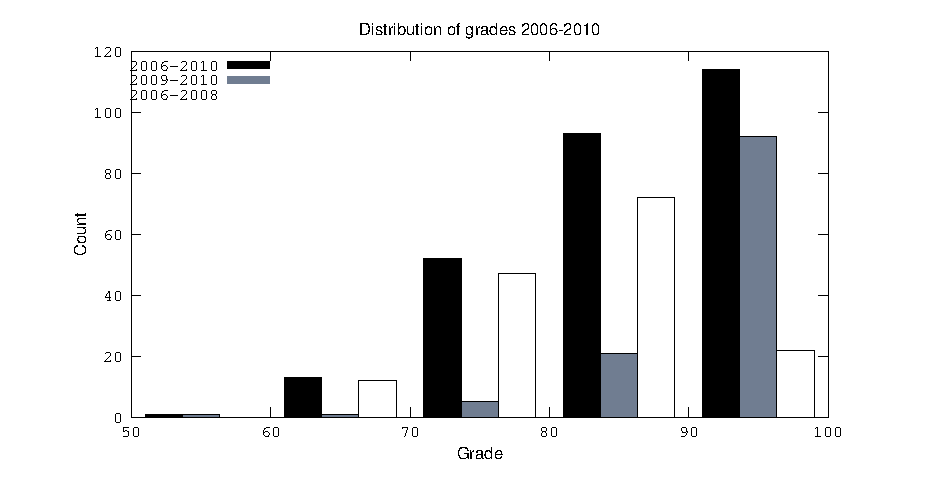
\includegraphics[width=0.8\linewidth]{526gradeDist}
\end{centering}

\section{Textbook}

There is no required textbook for this course. The lecture notes are
fairly detailed and self-contained (and become more so each
year). Nonetheless, additional references could be useful.

The notes were originally largely based on \textit{Mathematics for
  Economists} by \cite{sb1994}. However, over time the content has
diverged quite a bit. Nonetheless, Simon and Blume remains an okay
reference. Compared to the notes, Simon and Blume place less emphasis
on proofs and more emphasis on examples and exercises.

\textit{Optimization in economic theory} by \cite{dixit1990} is very
readable. It lacks rigorous proofs, but does a great job of conveying
the intuition for results. It also contains many economic
examples. This book would be useful for the first half of the course,
but not very useful for the second half.

\textit{Mathematical methods and models for economists} by
\cite{fuente2000} is a good middle ground between the practicality of
\cite{dixit1990} and \cite{sb1994} and the abstraction of
\cite{carter2001} and the other books listed below. I have only
recently come across it and not read it in detail, but it might be the
best choice for this course.

\textit{Foundations of Mathematical Economics} by \cite{carter2001} is
an excellent book, but is more difficult than the others listed
above. It contains many proofs and can be quite abstract. However, it
does do a good job of motivating everything with economic examples. I
especially recommend it if you have a solid mathematics background or
plan to continue studying economics after the MA program. Similar
books that could be used instead include \textit{Real analysis with
  economic applications} by \cite{ok2007} and \textit{An introduction
  to mathematical analysis for economic theory and econometrics} by
\cite{corbae2009}. These books are perhaps slightly more difficult
than \cite{carter2001}. \cite{corbae2009} would be especially useful
if you are interested in econometric theory because it contains an
excellent chapter on measure spaces and probability (topics that will
not be covered in this course).
 
The notes contain additional references that are relevant for specific
topics.

\section{Course Outline}

This course has two main goals. One is to introduce some mathematical
techiniques that will be useful in other courses. The second is to
develop comfort with the sort of higher level mathematics that is used
throughout economics. 

The first half of the course focuses on optimization. Economics is
largely about how to best allocate scarce resources. Consumers
maximize utlity subject to a budget constraint, firms maximize profits
subject to a production possibilities constraint, and the social
planner maximizers welfare subject to a resource constraint. You are
likely already familiar with finite dimension constrained
optimization. However, you might not be familiar with optimization in
infinite dimension. Infinite dimensional optimization problems appear
in economics when individuals have to choose something at every
instant of time or in every state of the world. The first few weeks of
the course will focus on solving optimization problems, including
those in inifinite dimension. 

After the midterm, we will take a step back rigorously prove some of
the results that we have been using. In particular, we will cover some
basic real analysis and calculus on vector spaces. This part of the
course is more abstract. The relevance of the mathematics that we
cover to economics will not always be apparent. However, rest assured
that what we cover is foundational and is essential for some areas of
economics, particularly theoretical econometrics, micro, and macro. 

\begin{enumerate}
\item Optimization
  \begin{enumerate}
  \item Constrained optimization
  \item Comparative statics
  \item The maximum principle
  \item Dynamic programming
  \end{enumerate}
\item Sets and numbers
\item Linear algebra
  \begin{enumerate}
  \item Systems of linear equations 
  \item Matrix Algebra 
  \item Eigenvalues, eigenvectors, and definite matrices 
  \item Vector spaces
  \end{enumerate}
\item Calculus on vector spaces
  \begin{enumerate}
  \item Basic topology 
  \item Differential calculus 
  \item Inverse and implicit functions
  \item Optimization on vector spaces
  \end{enumerate}
\item Convexity and the separating hyperplane theorem
\item Comparative statics without differentiability: supermodularity
  and topkis's theorem 
\end{enumerate}
It is possible that we will not have time to cover all topics,
especially the last two.

\section{Motivation and Goals}

Look through the most recent issues of the top economics journals (the
top five journals are
{\slshape{\href{http://onlinelibrary.wiley.com/journal/10.1111/(ISSN)1468-0262}{Econometrica},
  \href{https://www.aeaweb.org/journals/aer}{American Economic
    Review}, \href{http://qje.oxfordjournals.org/}{Quarterly Journal
    of Economics},
  \href{http://www.journals.uchicago.edu/toc/jpe/current}{Journal of
    Political Economy}, and
  \href{http://restud.oxfordjournals.org/content/current}{Review of
    Economic Studies}}}
). (i) In how many of the articles can you
understand the statement of the main results? (ii) How many of the proofs
could you have written yourself?  (iii) How many of the proofs can you
understand? (iv) How many of the proofs do you think you could figure out
with the help of many hours of work and consulting additional
references? I hope that after this course, the answers to these
questions are (i) most, (ii) a few, (iii) half or more, (iv) most. 

To be more specific, I looked at a handful of articles from the most
recent (in September 2016) issues of {\slshape{Econometrica}} and
{\slshape{ReStud}}. Here is what I thought.
\begin{itemize}
\item \cite{tirole2016} ``From Bottom of the Barrel to Cream of the
  Crop: Sequential Screening With Positive Selection'' is a paper that
  you should be able to understand quite well after this course. This
  paper looks at an optimal contracting problem that is somewhat
  similar to what we will look at with optimal control. 
\item \cite{rs2016} ``Optimal Taxation with Rent-Seeking'' is another
  paper that you should be able to understand quite well after this
  course. Section 2 is mostly finite dimensional optimization and may
  be familiar already, albeit with lots of tedious
  derivations. Sections 3 and 4 are related to optimal control.
\item \cite{mr2016} ``Robust Contracts in Continuous Time'' is also
  about optimal contracting, so it is related to what we will
  cover. However, this paper uses stochastic calculus, which we will
  not cover. I hope the course will provide enough information to
  understand the general idea of this paper, but understanding all the
  details will require further study. 
\item \cite{am2016}, ``Conditional Inference With a Functional
  Nuisance Parameter'' is a difficult econometrics paper. I hope this
  course will make this paper somewhat more approachable, but
  understanding this paper fully will still require lots of additional
  work.
\end{itemize}
My hope is that by the end of this course, you can look at any
economics paper and, at worst, say to yourself, ``with enough time and
effort, I can figure this out if needed.'' 


\clearpage
\bibliographystyle{jpe}
\bibliography{../526}

\end{document}

